\documentclass{beamer}
\usepackage{graphicx}
\usepackage{booktabs}
\usepackage[utf8]{inputenc}
\usepackage[english]{babel}
\usepackage{xcolor}
\usepackage[export]{adjustbox}
\usepackage{listings}
\definecolor{mygreen}{rgb}{0,0.6,0}
\definecolor{mygray}{rgb}{0.5,0.5,0.5}
\definecolor{mymauve}{rgb}{0.58,0,0.82}
\lstset{ 
  backgroundcolor=\color{white},   % choose the background color; you must add \usepackage{color} or \usepackage{xcolor}; should come as last argument
  basicstyle=\footnotesize,        % the size of the fonts that are used for the code
  breakatwhitespace=false,         % sets if automatic breaks should only happen at whitespace
  breaklines=true,                 % sets automatic line breaking
  captionpos=b,                    % sets the caption-position to bottom
  commentstyle=\color{mygreen},    % comment style
  deletekeywords={...},            % if you want to delete keywords from the given language
  escapeinside={\%*}{*)},          % if you want to add LaTeX within your code
  extendedchars=true,              % lets you use non-ASCII characters; for 8-bits encodings only, does not work with UTF-8
  firstnumber=1000,                % start line enumeration with line 1000
  frame=single,	                   % adds a frame around the code
  keepspaces=true,                 % keeps spaces in text, useful for keeping indentation of code (possibly needs columns=flexible)
  keywordstyle=\color{blue},       % keyword style
  language=Octave,                 % the language of the code
  morekeywords={*,...},            % if you want to add more keywords to the set
  numbers=left,                    % where to put the line-numbers; possible values are (none, left, right)
  numbersep=5pt,                   % how far the line-numbers are from the code
  numberstyle=\tiny\color{mygray}, % the style that is used for the line-numbers
  rulecolor=\color{black},         % if not set, the frame-color may be changed on line-breaks within not-black text (e.g. comments (green here))
  showspaces=false,                % show spaces everywhere adding particular underscores; it overrides 'showstringspaces'
  showstringspaces=false,          % underline spaces within strings only
  showtabs=false,                  % show tabs within strings adding particular underscores
  stepnumber=2,                    % the step between two line-numbers. If it's 1, each line will be numbered
  stringstyle=\color{mymauve},     % string literal style
  tabsize=2,	                   % sets default tabsize to 2 spaces
  title=\lstname                   % show the filename of files included with \lstinputlisting; also try caption instead of title
}

\definecolor{dg}{RGB}{45,187,45}

\title[SMOG-1]
{
	\color{red} PocketQube Class Student Satellites in Hungary\\
	\medskip
	\normalsize \color{dg} "The Smallest Operational Satellites in the World with scientific on-board payload."
}
\author{Levente Dudás, András Gschwindt}
\institute[BME VIK SzHVT]{
	\medskip
	\color{purple} \normalsize \textit{dudas.levente@vik.bme.hu}\\
	\medskip
	\large \color{blue}\url{https://gnd.bme.hu}
}
\date{\today}

\begin{document}

\newcommand{\slidetime}{60}

\begin{frame}
\transduration{\slidetime}
\begin{center}

\includegraphics[width=1.0\textwidth]{hvt.jpg}
\end{center}
\titlepage
\end{frame}

\section{SMOG}
\begin{frame}
\transduration{\slidetime}
\frametitle{SMOG-1 \& SMOG-P}
\begin{enumerate}
\item DVB-T band Spectrum Monitor.
\item Measurement of Total Ionising Dose.
\item Application of hysteresis material to decrease orbit lifetime.
\end{enumerate}

\centering{Single-point failure tolerant, cold-redundant on-board satellite sub-systems with local intelligence.}

\begin{columns}
\column{.5\textwidth}
\begin{itemize}
	\item 50 x 50 x 50 mm
	\item 183 g mass
	\item $-40 ... +80 C$ temp. range
	\item $~20 g$ acc. load
	\vspace{3mm}
	\item 06.12.2019, Electron - SMOG-P
	\item 22.03.2021, Soyuz - SMOG-1
\end{itemize}
\column{.5\textwidth}
\begin{figure}
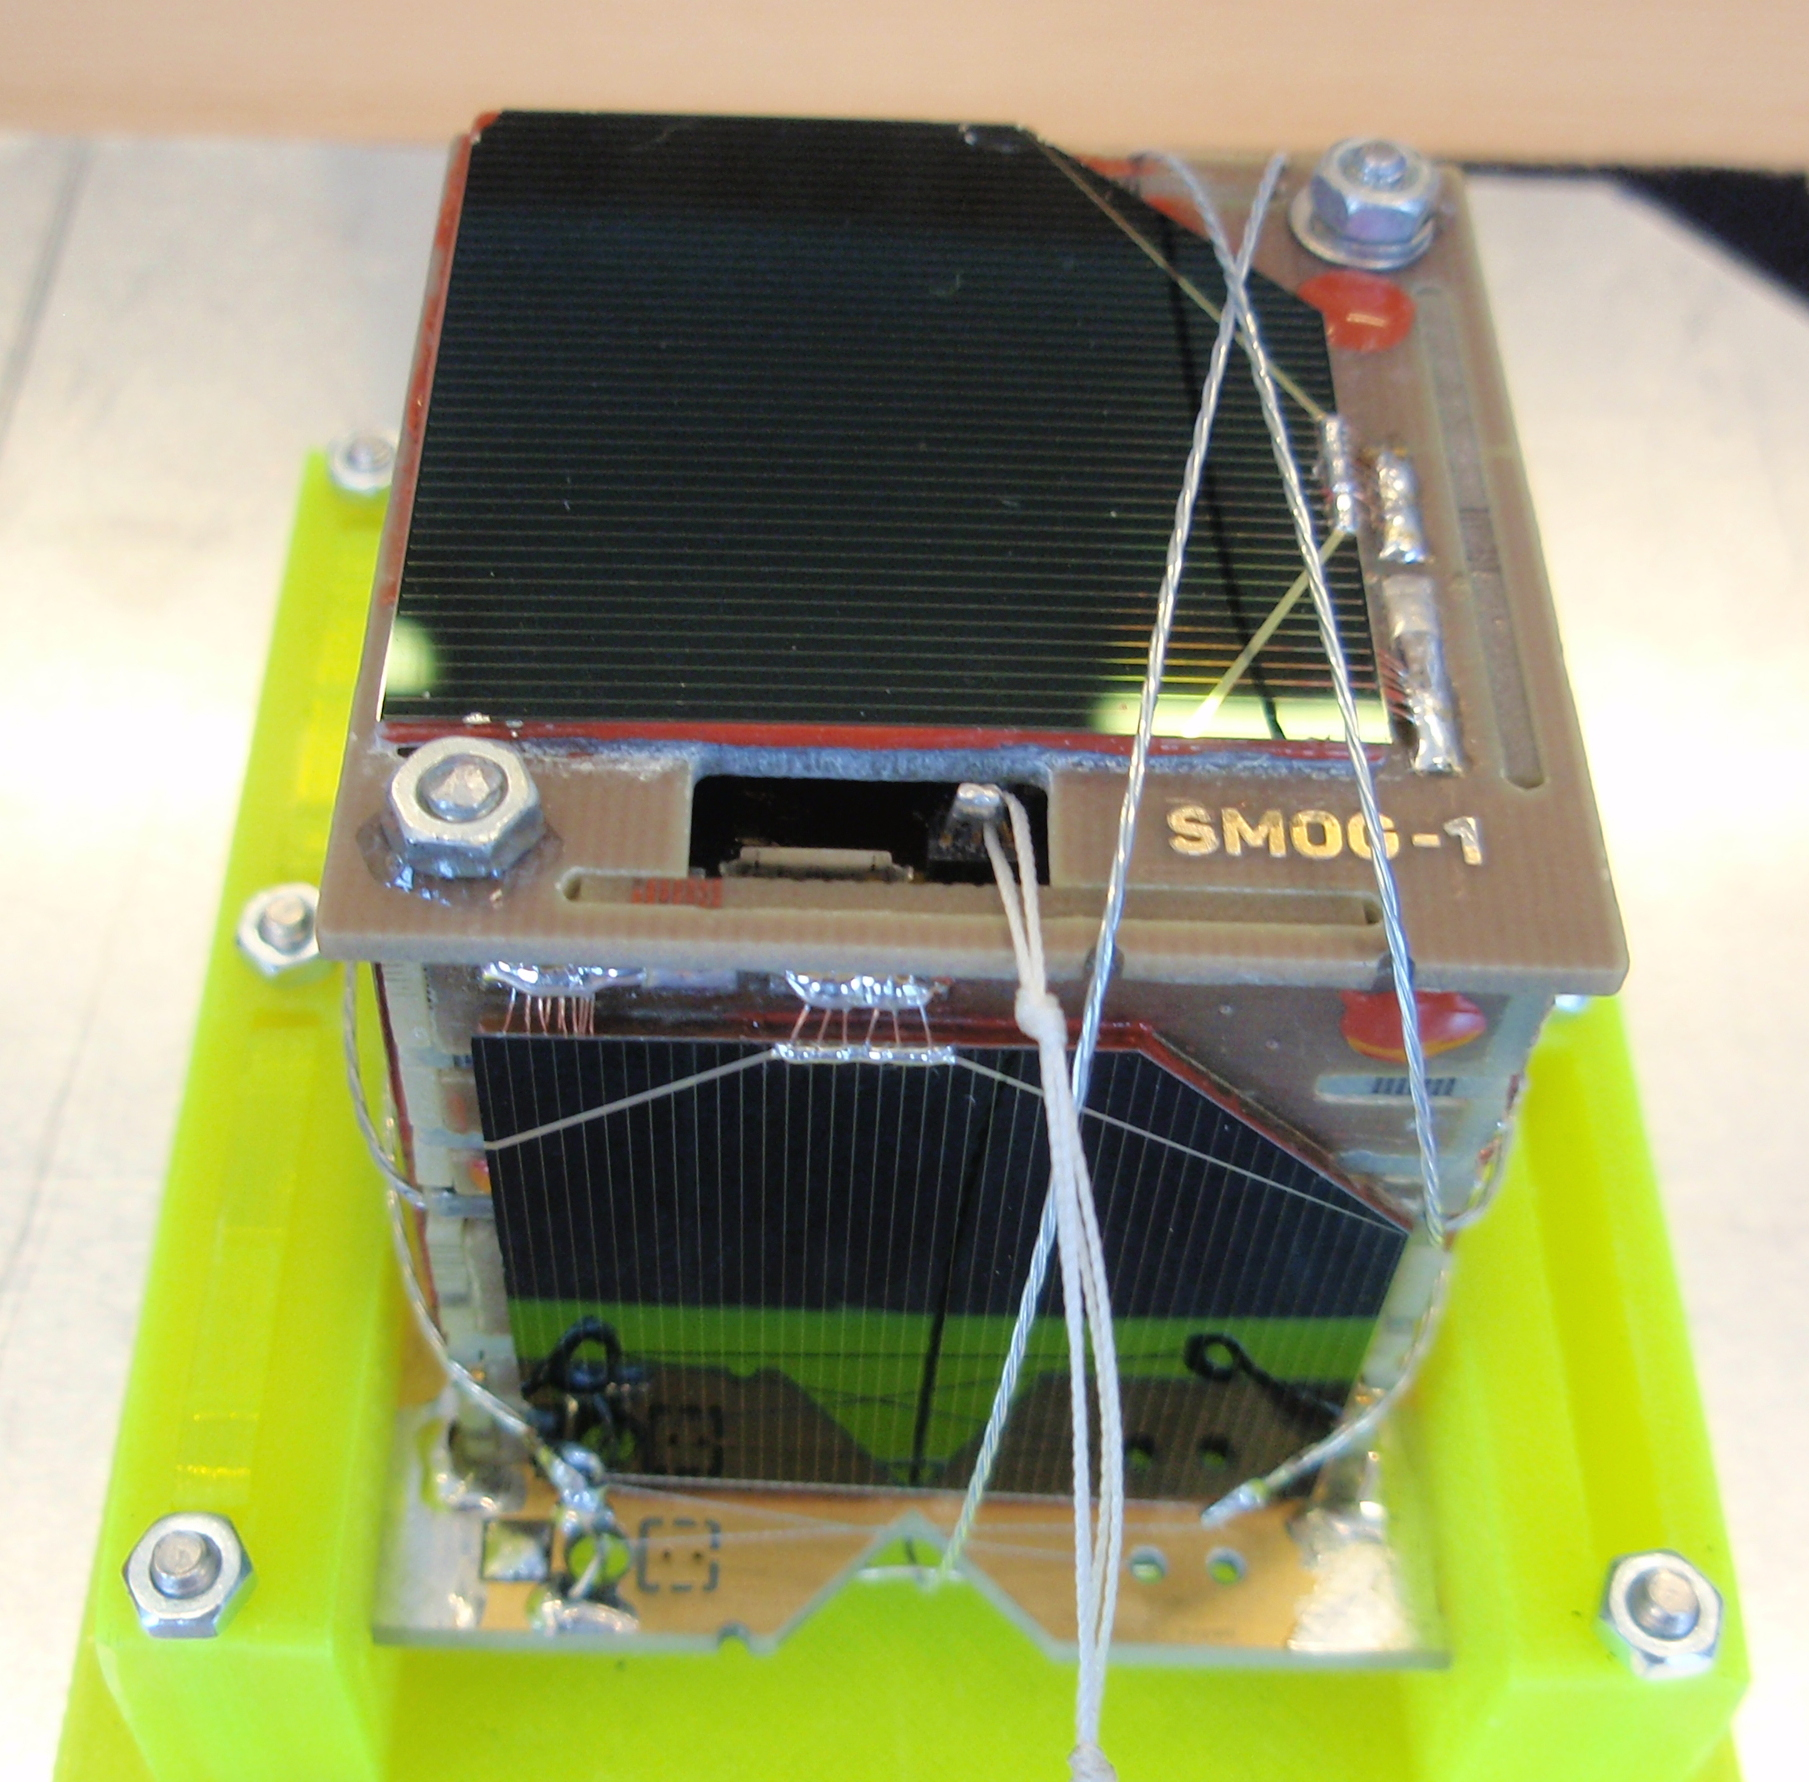
\includegraphics[width=50mm]{P9060082.JPG}
\end{figure}
\end{columns}
\end{frame}

\begin{frame}
\transduration{\slidetime}
\frametitle{Global DVB-T Band Electromagnetic Pollution Map}
\centering
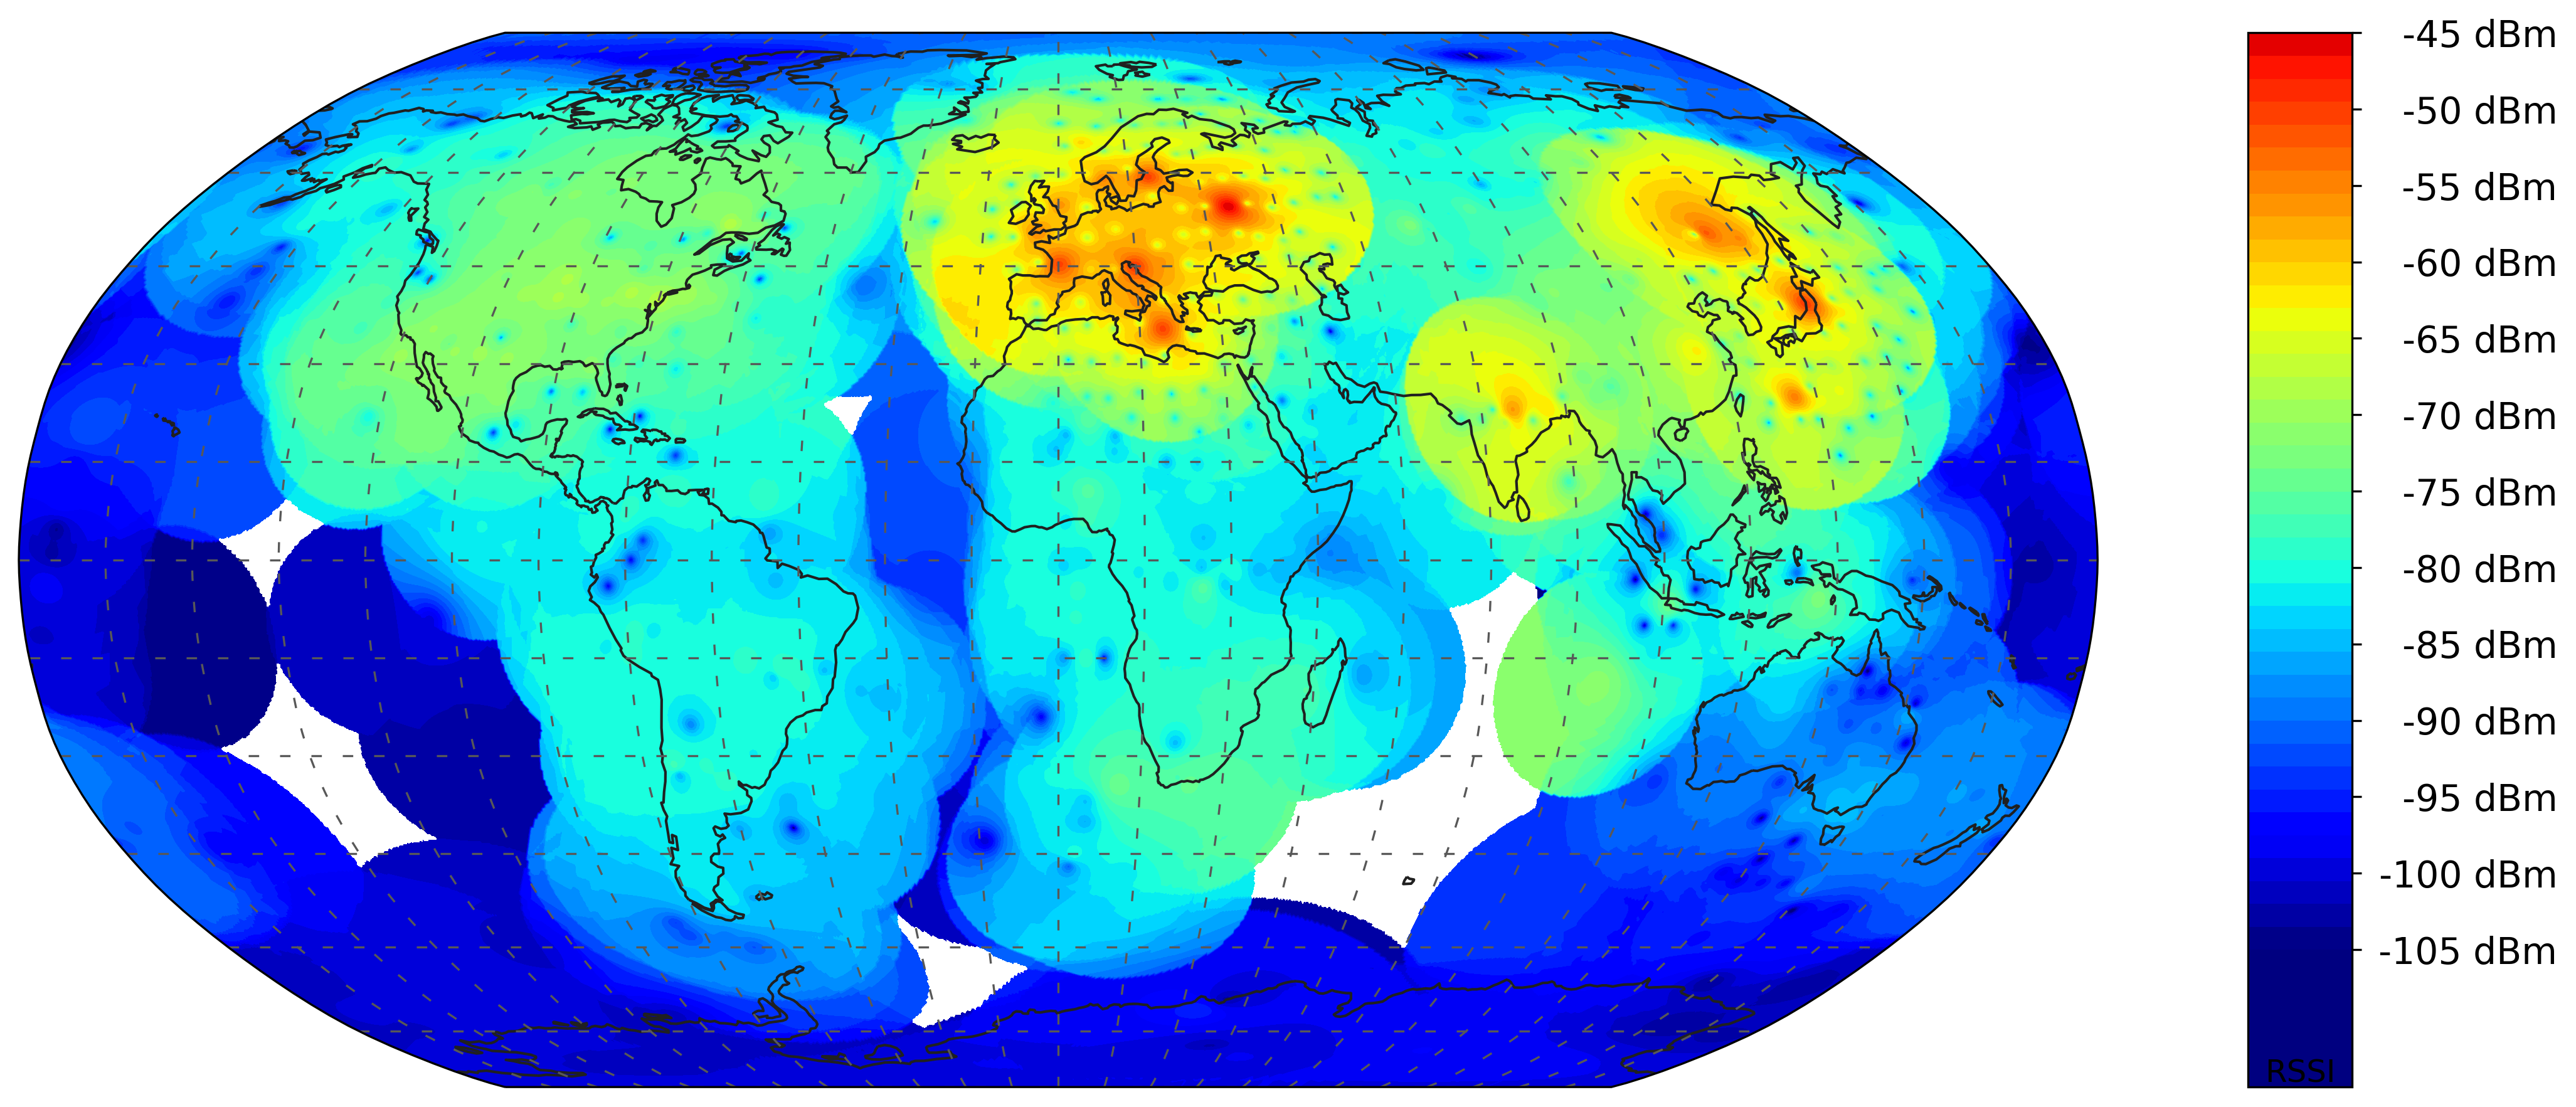
\includegraphics[width=1.05\textwidth]{pollution_map.png}\\
Donát Takács, Boldizsár Markotics - BME VIK TDK 2020\\
\end{frame}

\begin{frame}
\transduration{\slidetime}
\frametitle{This is a source code here.}
\centering
\lstinputlisting{while1.c}
\end{frame}

\begin{frame}
\transduration{\slidetime}
\frametitle{This is a block scheme here.}
\centering
Compile \textit{gmsk\_dem.tex} file, then include \textit{gmsk\_dem.pdf}.

\vspace{5mm}
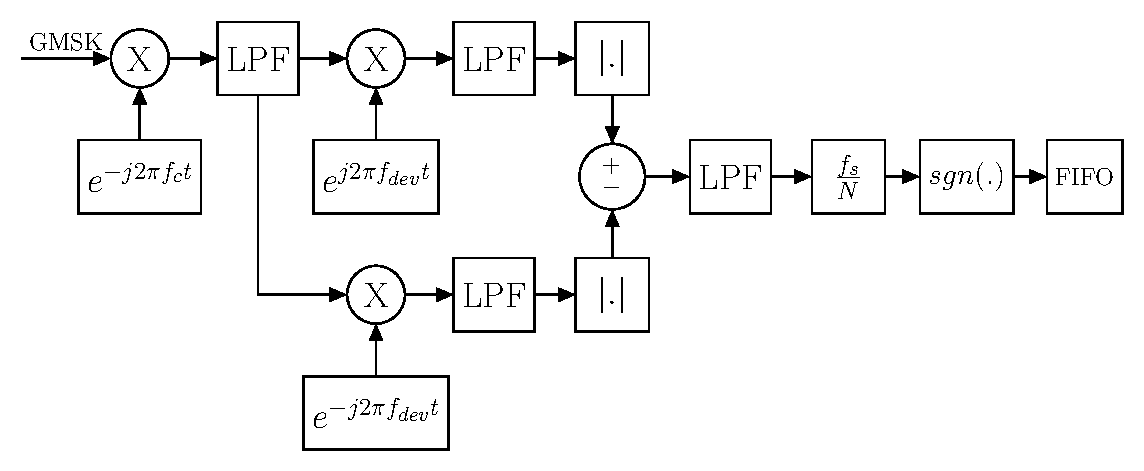
\includegraphics[width=1.0\textwidth]{gmsk_dem.pdf}
\end{frame}

\section{End}
\begin{frame}
\transduration{600}
\centering
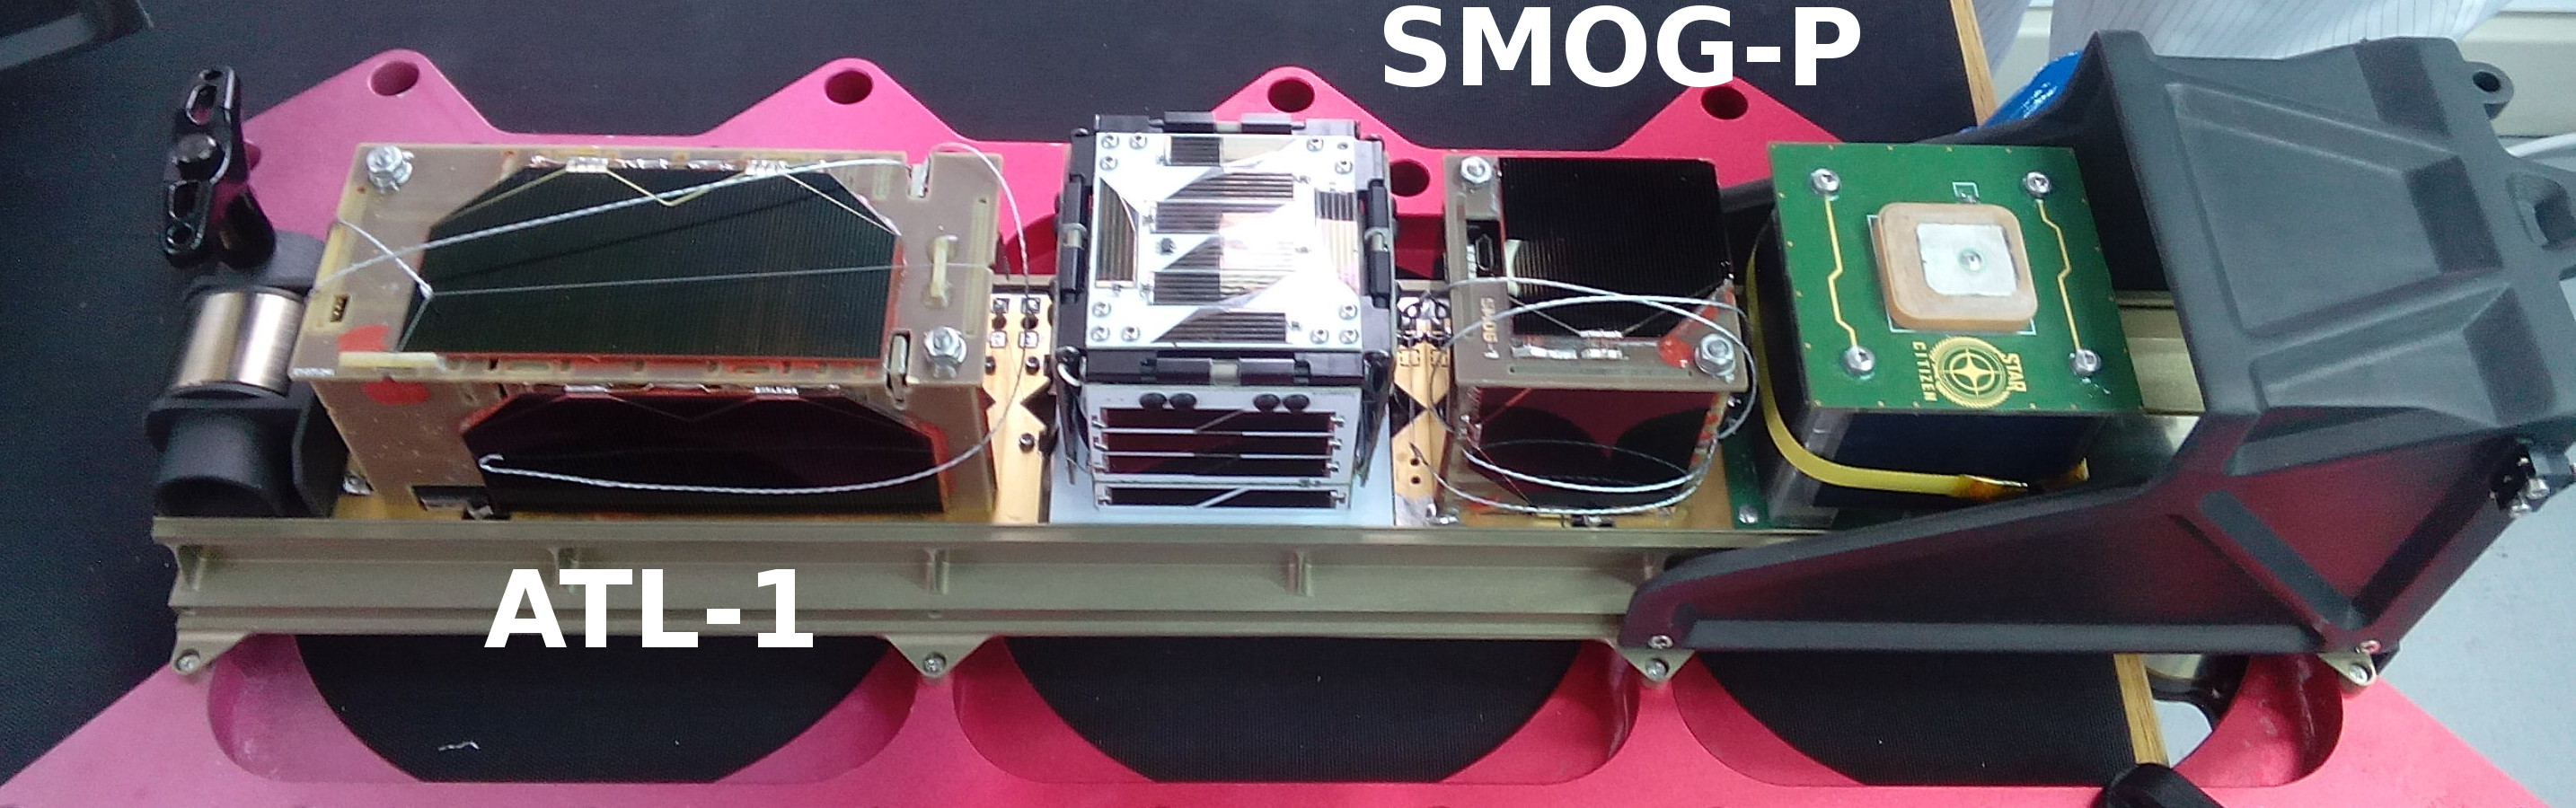
\includegraphics[width=1.0\textwidth]{albapod.jpg}\\
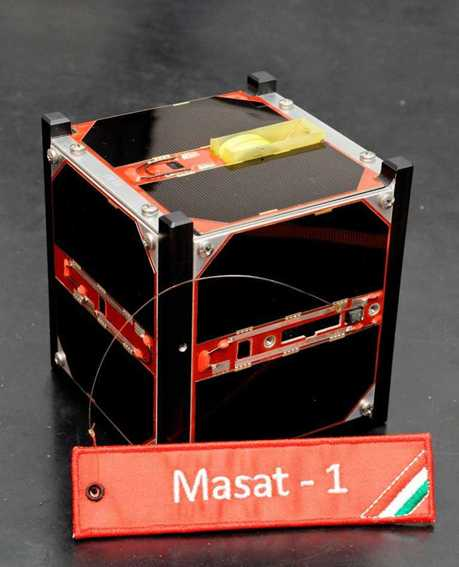
\includegraphics[width=0.335\textwidth]{masat1.jpg}
\hspace{5mm}
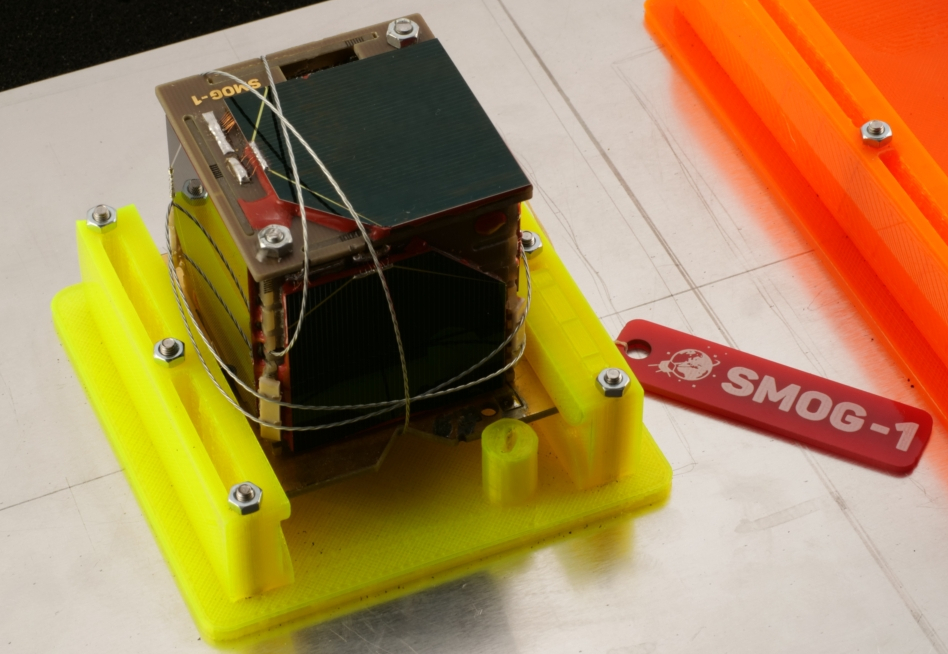
\includegraphics[width=0.58\textwidth]{smog1ready.jpg}\\
Operated: \color{blue}Masat-1, SMOG-P, ATL-1\color{black}; operational: \color{red}SMOG-1
\end{frame}


\end{document}


